\chapter{Implementation and Testing}

SEDS was developed using six 2-week Agile sprints, with incremental delivery of core functionality: (1) admin authentication and station/zone management, (2) citizen SOS with guest auto-provisioning, (3) responder dispatch queue with atomic claiming, (4) real-time lifecycle notifications via SSE + Redis. All core objectives have been implemented, tested, and integrated.

\section{Implementation}

\subsection{Tools Used}

\subsubsection{CASE Tools and Development Environment}

\begin{table}[H]
\centering
\caption{Development Tools and Platforms}
\rowcolors{1}{gray!10}{white}
\begin{tabularx}{\textwidth}{|X|X|X|}
\hline
\textbf{Category} & \textbf{Tool} & \textbf{Purpose} \\
\hline
Editor & VS Code & Code editing, debugging, ESLint/Prettier integration \\
\hline
Version Control & GitHub & Repository, CI/CD via GitHub Actions (linting, type check, test) \\
\hline
Linting/Formatting & ESLint, Prettier & Code quality and consistency \\
\hline
Testing & Postman, Manual & API endpoint and end-to-end flow testing \\
\hline
Containerization & Docker, Docker Compose & Service orchestration (frontend, backend, postgres, redis) \\
\hline
\end{tabularx}
\label{tab:tools}
\end{table}

\subsubsection{Programming Languages and Frameworks}

Frontend: TypeScript 5 with Next.js 16 (App Router), React 19, MapLibre GL JS 3.x, Zustand, React Hook Form + Zod, TailwindCSS 4, shadcn/ui.

Backend: Node.js 20, TypeScript 5, Express.js 4, Sequelize ORM 6, bcrypt, jsonwebtoken (JWT), Nodemailer, google-auth-library.

\subsubsection{Database Platforms}

PostgreSQL 16 with PostGIS 3.4 extension (spatial geometry, GIST indexing). Redis 7 Alpine (pub/sub broker).

\subsection{Implementation Details of Modules}

\subsubsection{Frontend Architecture}

\textbf{Development Phases (Sprints 1–6):}

Sprint 1--2: Authentication (JWT signup/login/OAuth2), responder account management, station/zone CRUD with MapLibre GL polygon drawing.

Sprint 2--3: Guest user auto-provisioning, SOS request form, geolocation API integration, location picker, status modal.

Sprint 3: Responder dashboard queue view, radar visualization (pulsing rings), atomic claim button, polling refresh.

Sprint 4--6: Real-time SSE streams, incident lifecycle buttons (Arrive, Resolve), responder action transitions, SSE reconnection with polling fallback.

\textbf{Key Components:} Landing page with interactive map (stations + zones), Emergency Button modal (geolocation + SOS form), Responder dashboard (queue view + current task + radar visualization), Admin interface (station/responder/zone CRUD via MapLibre GL drawing tools).

\begin{figure}[H]
  \centering
  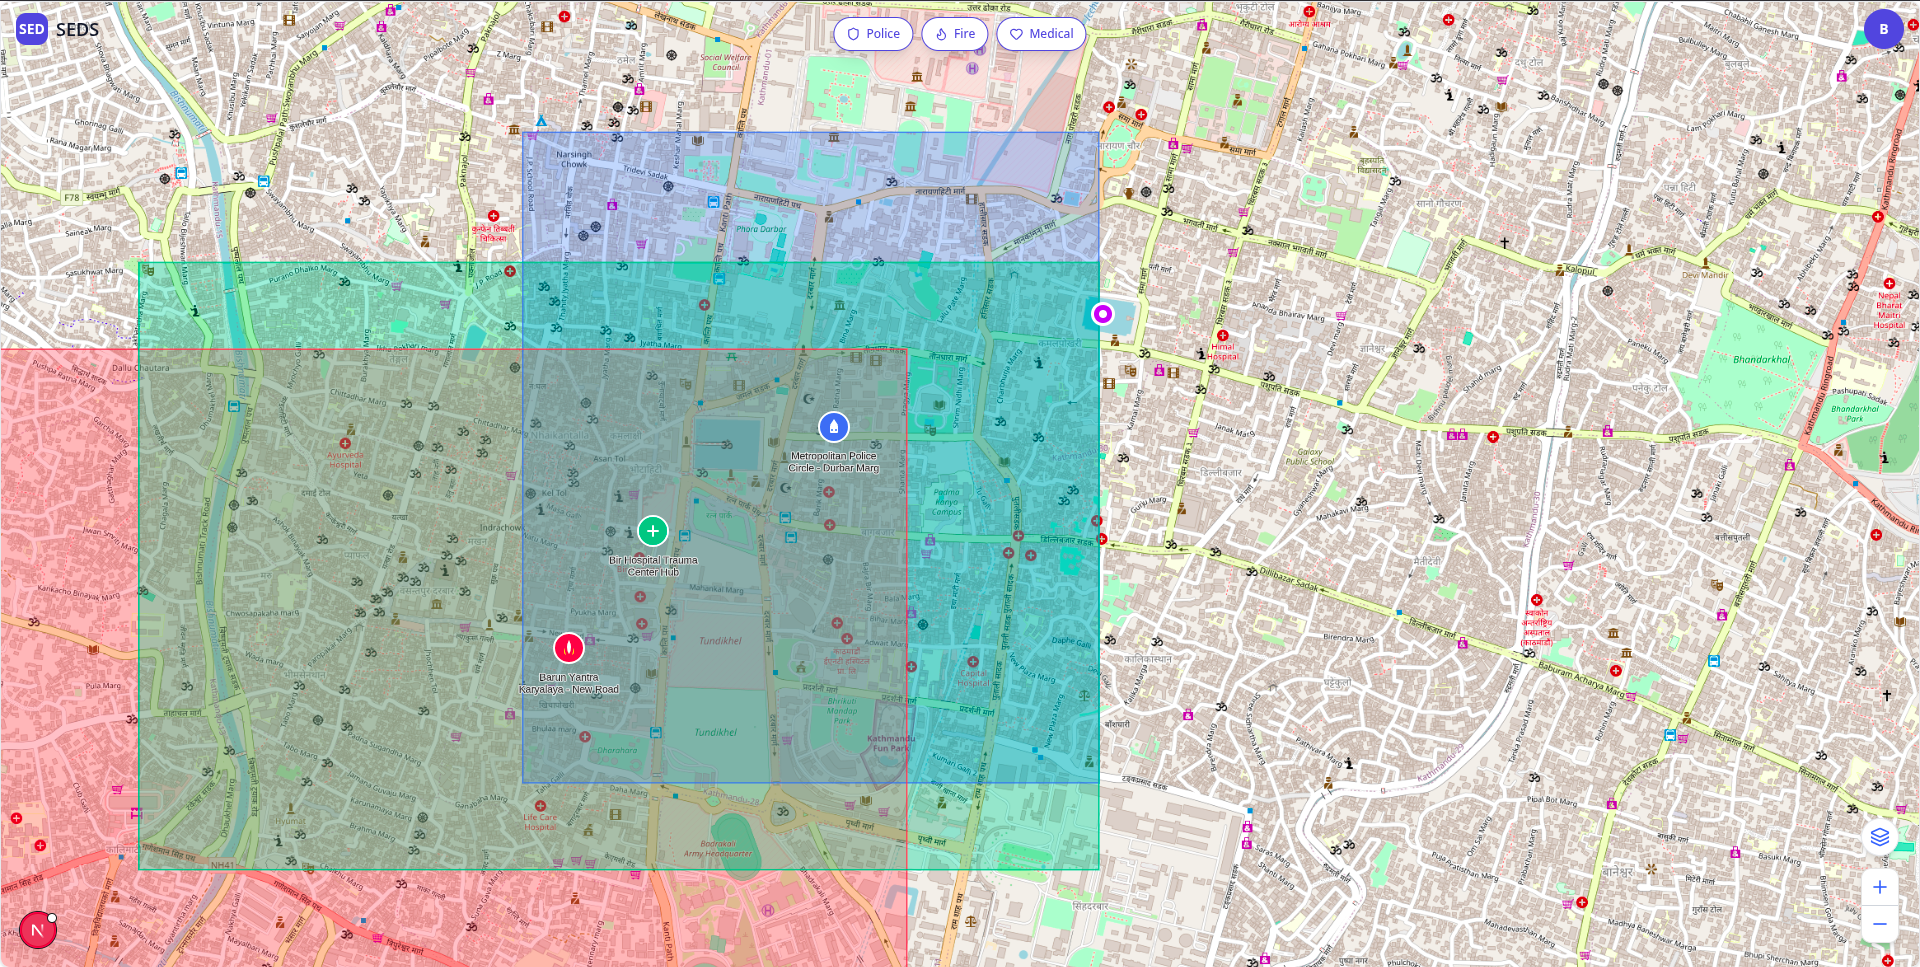
\includegraphics[width=\textwidth]{Graphics/landing-page.png}
  \caption{Landing Page - Interactive map with stations and service zones}
  \label{fig:landing}
\end{figure}

\begin{figure}[H]
  \centering
  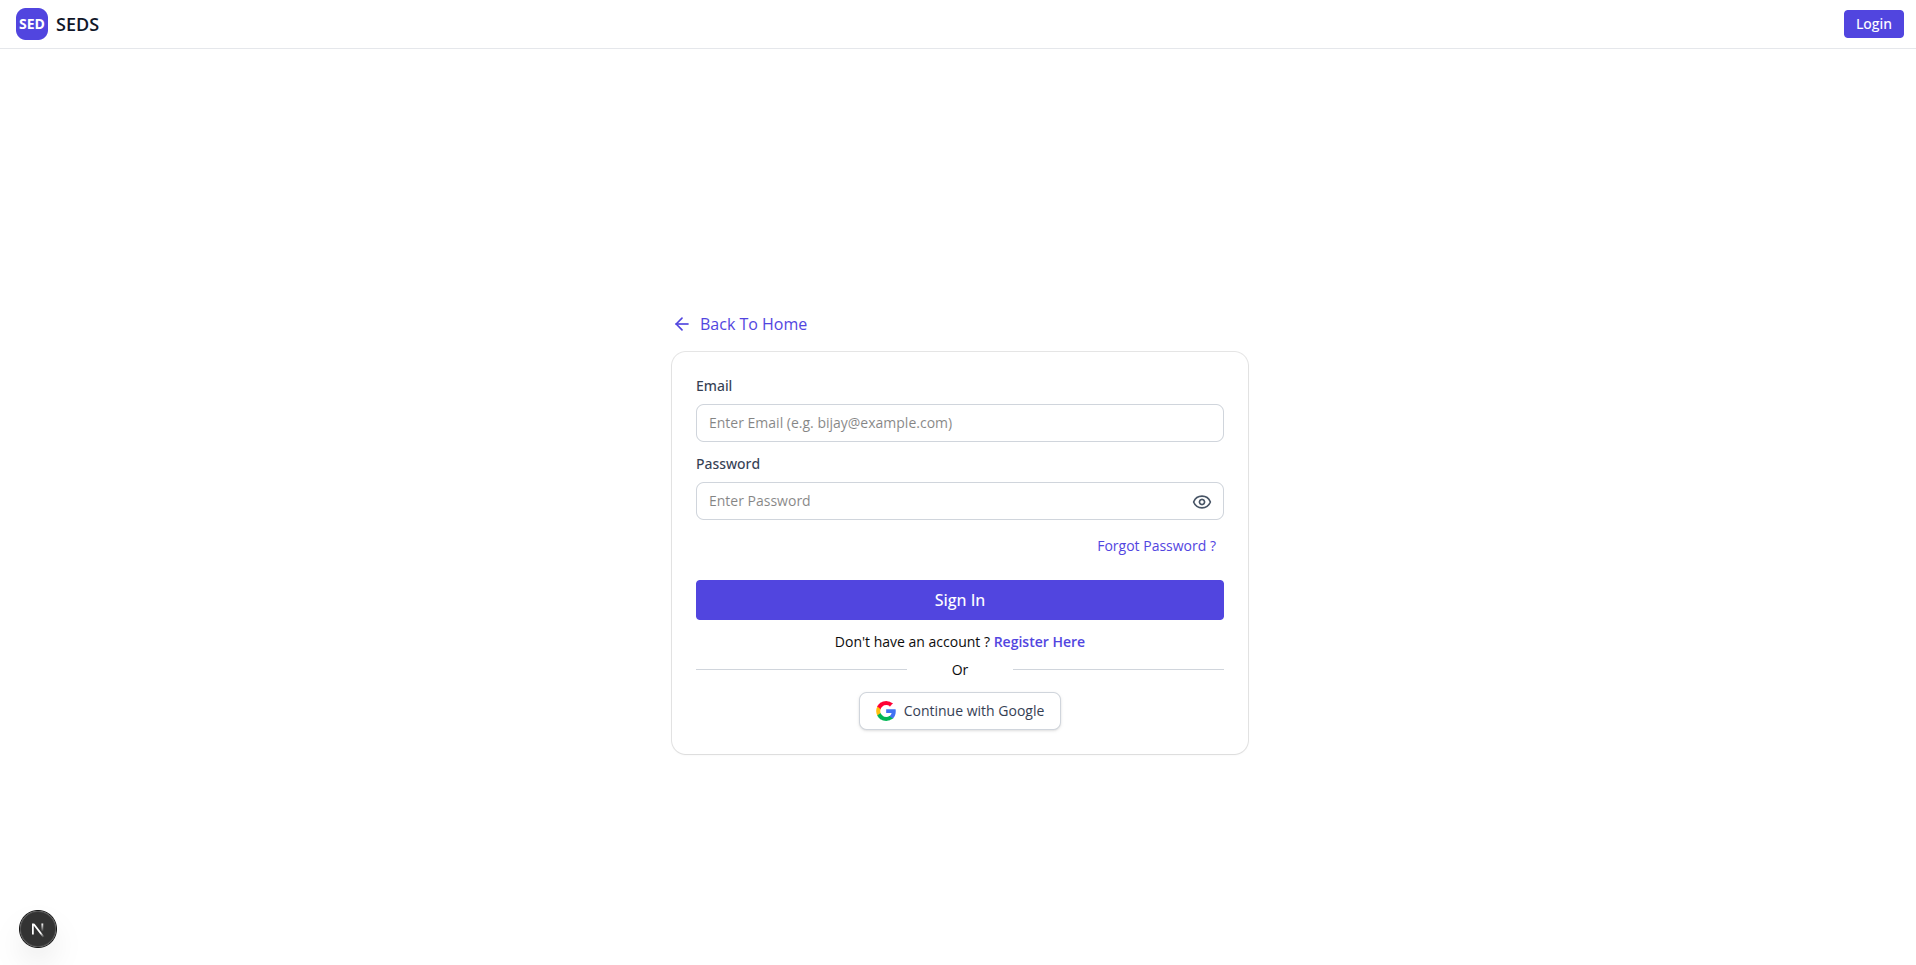
\includegraphics[width=\textwidth]{Graphics/login-page.png}
  \caption{Login Page - Role-based authentication (Admin/Responder)}
  \label{fig:login}
\end{figure}

\FloatBarrier

\begin{figure}[H]
  \centering
  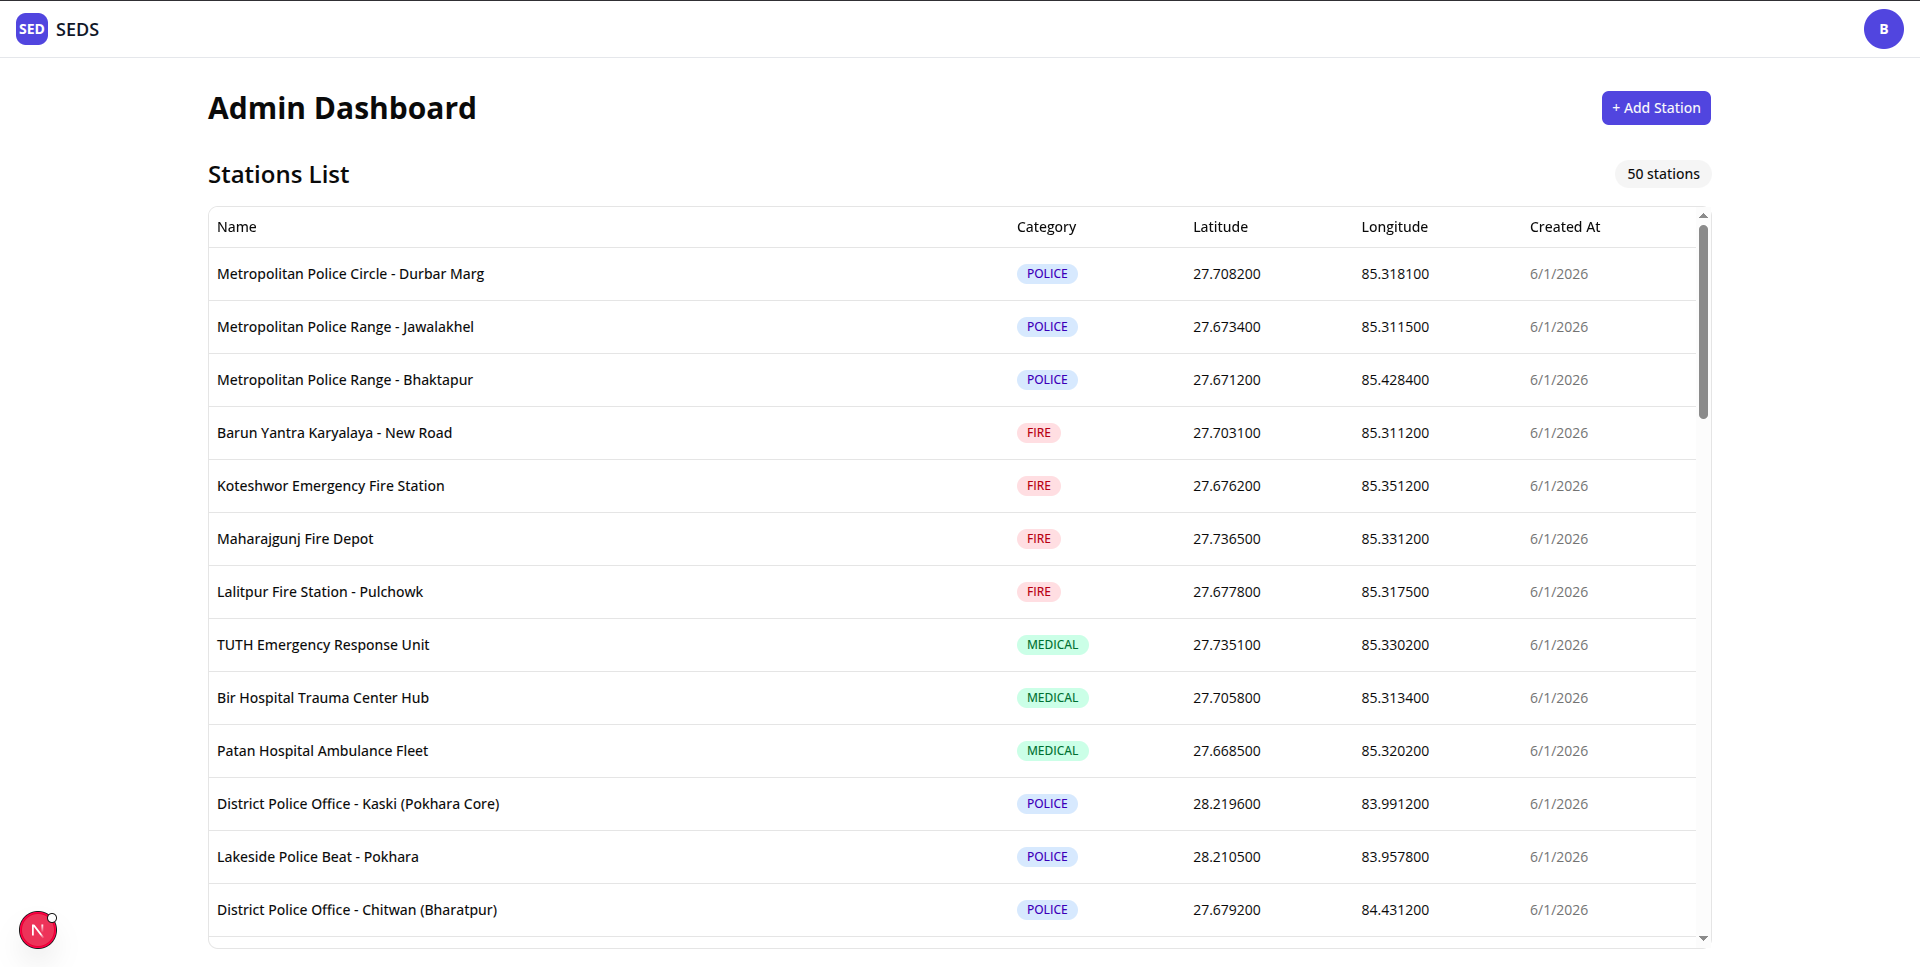
\includegraphics[width=\textwidth]{Graphics/admin-dashboard.png}
  \caption{Admin Dashboard - Station management with CRUD operations}
  \label{fig:dashboard}
\end{figure}

\begin{figure}[H]
  \centering
  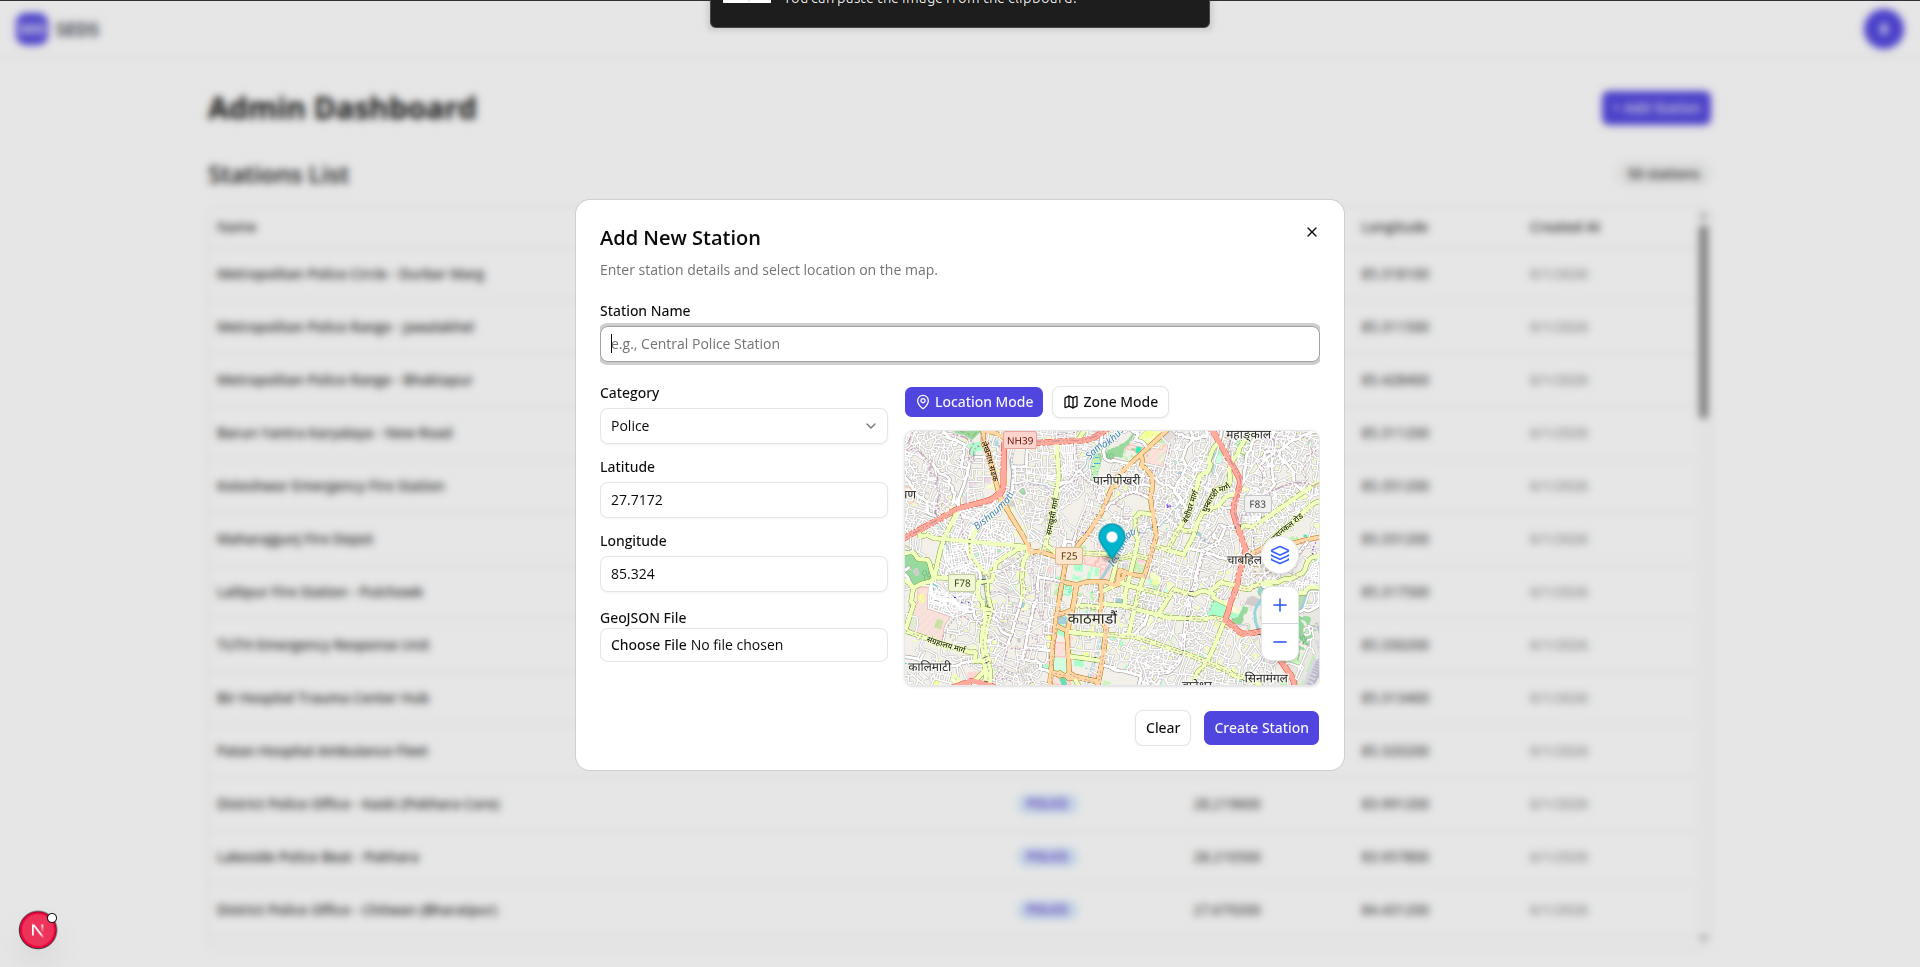
\includegraphics[width=\textwidth]{Graphics/add-station-form.png}
  \caption{Add Station Form - Location picker and zone polygon drawing}
  \label{fig:addstation}
\end{figure}

\FloatBarrier

\subsubsection{Backend REST API}

The API is organized under \texttt{/api/v1/} with role-based middleware (authenticate, maybeAuthenticate, isAdmin, isResponder).

\textbf{Core Endpoints:} Authentication (signup, login, OAuth), incident CRUD and lifecycle transitions, station and responder CRUD (admin), SSE stream (real-time updates), atomic claim with row-level locking.

\subsubsection{Database Implementation}

PostgreSQL 16 with PostGIS 3.4. Sequelize ORM manages schema via migrations. Key spatial queries:

\textbf{Zone Containment Query:} Uses PostGIS \texttt{ST\_Contains()} to check if incident location falls within any zone boundary. Returns the station if match found; else returns null.

\textbf{Nearest Station Fallback:} Uses PostGIS \texttt{ST\_Distance()} to compute Haversine distance from incident location to each station. Returns the closest station.

\textbf{Atomic Claim Transaction:}

\begin{verbatim}
BEGIN;
SELECT * FROM incidents WHERE id = ? FOR UPDATE;
UPDATE incidents SET status = 'RESPONDING',
  responder_id = ?, accepted_at = NOW() WHERE id = ?;
UPDATE responders SET status = 'BUSY' WHERE id = ?;
COMMIT;
\end{verbatim}

The \texttt{FOR UPDATE} lock serializes concurrent attempts; if the responder is already busy, the transaction aborts with a constraint violation or explicit 409 check.

\subsubsection{Real-Time Communication}

\textbf{SSE + Redis Pub/Sub Model:}

Controllers publish incident events to Redis channels named \texttt{station:\{station\_id\}} and \texttt{citizen:\{user\_id\}}. The sseService.ts layer subscribes and pushes messages to connected EventSource clients.

\textbf{Citizen Flow:} Citizen submits SOS; incident created and published to Redis citizen channel; SSE push to citizen's browser ("Help is on the way" within 1 second).

\textbf{Responder Flow:} New incident at station; published to Redis station channel; SSE push to all responders; UI auto-opens queue modal; responder clicks Claim; atomic lock prevents double-claim; incident status becomes RESPONDING.

\textbf{Fallback:} SSE disconnect; clients poll GET /incidents/active every 5 seconds; status caught up within 5 seconds with no missed updates.

\subsubsection{Concurrency Control}

Row-level locking (SELECT ... FOR UPDATE) ensures only one responder can claim an incident. Early implementation locked without fetching, causing Postgres errors on concurrent claims. Solution: fetch the incident row (while locked) to validate preconditions, then update atomically. Testing: 10 concurrent responders on 100 incidents → zero double-claims; single incident claimed by 10 concurrent requests → 1 success, 9 failures (409).

\subsubsection{Security Implementation}

\begin{itemize}
  \item bcrypt password hashing (10 salt rounds, OWASP compliant).
  \item JWT tokens issued in HTTP-only, Secure, SameSite=Strict cookies (CSRF + XSS protection).
  \item Role-based access control via middleware (isAdmin, isResponder checks on protected endpoints).
  \item Parametrized queries via Sequelize ORM (SQL injection prevention).
  \item Email verification required before responder account activation.
\end{itemize}

\section{Testing}

\subsection{Test Cases for System Testing}

\begin{table}[H]
\centering
\caption{System Testing - Authentication and Incident Lifecycle}
\rowcolors{1}{gray!10}{white}
\begin{tabularx}{\textwidth}{|X|X|}
\hline
\textbf{Test Case} & \textbf{Result} \\
\hline
Signup with email/password, login, JWT cookie set & Pass \\
\hline
SOS submission (POST /incidents) - incident created, station assigned & Pass \\
\hline
Atomic claim (PATCH /incidents/:id/claim) - responder assigned via lock & Pass \\
\hline
Concurrent claim (2 responders) - first succeeds (200), second fails (409) & Pass \\
\hline
Incident lifecycle: Pending → Responding → Arrived → Resolved & Pass \\
\hline
\end{tabularx}
\label{tab:sys-test-auth}
\end{table}

\begin{table}[H]
\centering
\caption{System Testing - Admin Operations and Access Control}
\rowcolors{1}{gray!10}{white}
\begin{tabularx}{\textwidth}{|X|X|}
\hline
\textbf{Test Case} & \textbf{Result} \\
\hline
Create station with zone - both created, 201 response & Pass \\
\hline
List stations, responders (GET /admin/stations, /admin/responders) & Pass \\
\hline
RBAC: POST /admin/stations as citizen - 403 Forbidden & Pass \\
\hline
SSE stream (GET /incidents/stream) - real-time updates via EventSource & Pass \\
\hline
\end{tabularx}
\label{tab:sys-test-admin}
\end{table}

\subsection{Result Analysis}

\subsubsection{Spatial Query Performance}

Zone containment (ST\_Contains) on 100 zones, 1000 incidents: average latency 2.3 ms (with GIST index). Nearest-distance fallback (ST\_Distance) on 20 stations: average latency 4.7 ms. Combined triage: average 6.5 ms per incident submission.

\subsubsection{Concurrent Claim Race Test}

10 responders, 100 incidents: zero double-claims across all trials (row-level locking effective). Single incident claimed by 10 concurrent requests: 1 success (200), 9 failures (409/400). No undefined state.

\subsubsection{SSE Reconnect Behavior}

Client SSE disconnect, backend running: client detects close, polls fallback immediately, reconnects within 2 seconds. No lost messages on 100-message test (verified via polling catch-up). Backend restart while client connected: SSE connection closes, client polls, backend recovers, reconnect succeeds.

\subsubsection{Real-Time Latency}

Status update publish → SSE push to all station responders: $< 100$ ms (Redis pub/sub + event loop). Polling refresh rate: 5 seconds, within tolerance for non-emergency updates.

\subsubsection{End-to-End Incident Flow}

Citizen submits SOS (location in zone): instant assignment, incident created ($< 50$ ms), SSE/polling push to responders ($< 100$ ms). Responder claims: atomic lock acquired, status updated to Responding, citizen notified via SSE ($< 100$ ms). Responder marks arrived/resolved: status transitions logged, both parties notified. Total flow (SOS to resolution): real-time responsive with $< 200$ ms cumulative backend latency.
